\section{Introduction}

Spline regression \citep{wahba1990spline, schumaker2007spline, gu2013smoothing} is a nonparametric method for modelling the complex dependencies between features, widely used in many fields including machine learning, econometrics and biomedicine. It is an ideal alternative to linear regression in the nonlinear data analysis. However, given the number and location of knots, the spline space is actually a linear space with a spline basis. Thus, the spline regression degenerates to a simple linear regression with respect to the basis, posing a strict limitation on its representative capacity. The ordinary solution is to assign sufficiently many knots and locate them uniformly, leading to a trade-off between the complexity and the flexibility of splines; see smoothing splines and thin plate splines \citep{10.1111/1467-9868.00374}. Furthermore, the splines with fixed knots usually assume each knot is used only once. This means the spline function has continuous derivatives up to its degree minus one. Consequently, it is inappropriate for the distinct-knot spline to fit curves with jumping discontinuity. %illustrated in Figure \ref{fig:spline}.

\iffalse
\begin{figure}
    \centering
    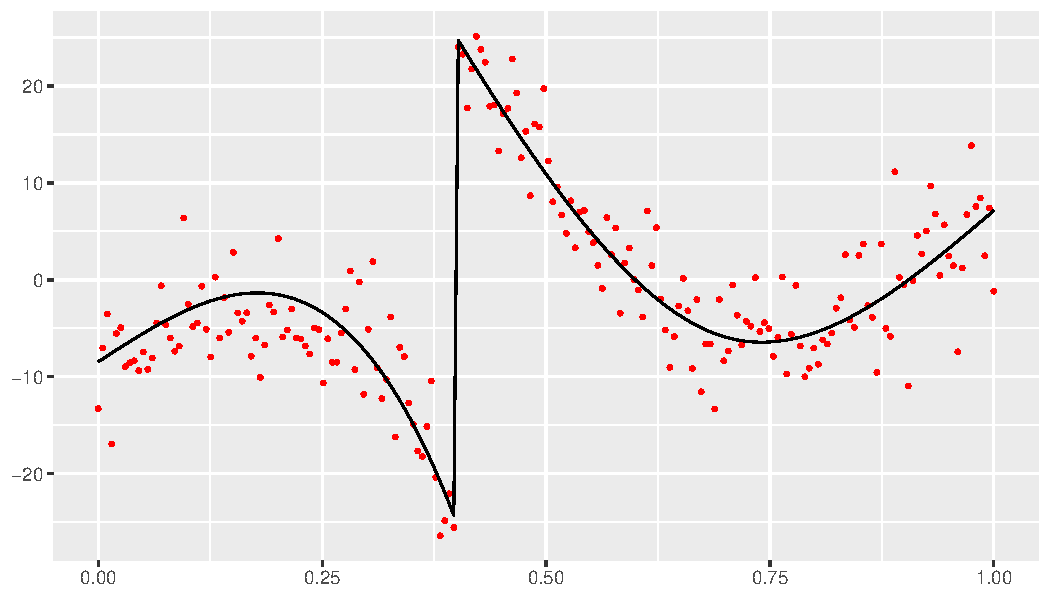
\includegraphics[width=0.5\textwidth]{Experiments/plots/spline_regression.pdf}
    \caption{A cubic spline with the jumping discontinuity at $0.4$.}
    \label{fig:spline}
\end{figure}
\fi

Rather than equally-spaced knots, we develop a Bayesian approach for the automatic selection of the spline knots. 
%In the multiple regression case, we utilize the tensor product spline \citep{dierckx1995curve} to make predictions.
% Rather than equally-spaced or quantile-based knots, we propose an extended Bayesian adaptive knot spline regression method (EBARS) to estimate the proper number and location of knots. 
The basic principle is modelling the intricate relationships with a few knots and the optimal location. The adaptive knot method reduces the complexity of splines when preserving the flexibility. We can also model the sharp changes by placing several knots in the almost coincident position. Moreover, the knot estimation provides a mechanism for easy interpretation. The number of knots detects how many transitions occur and the location indicates where change points lie. Thus, the quantities are of independent interest in many applications. For example, by examining the approval ratings of successful politicians, the president can determine the optimal time to switch from the job of governing to the job of running for reelection \citep{marsh2001spline}. See \citet{aminikhanghahi2017survey, truong2020selective} for a review about the change point detection in time series.

A considerable amount of work has been done for the knot selection. Some researchers rely on specialist knowledge or exploratory data analysis to specify the knots heuristically. But the ad hoc manner is rough since the exact knot information is unknown. \citet{10.2307/2346413} chose the knots via a grid-search method, whose search time grows exponentially with the increasing sample size. \citet{muggeo2003estimating} proposed a segmented regression method to estimate the break-point location based on a linearization technique and developed an R package \citep{muggeo2008segmented}. But this method is limited to linear splines and the number of knots is required to be known. For likelihood-based inference, the primary difficulty is that the likelihood is not differentiable with respect to the knots. Given the number of knots, \citet{doi:10.1080/01621459.2015.1073154} utilized local quadratic smoothing to approximate linear spline models and \citet{doi:10.1080/01621459.2021.1947307} proposed modified derivatives of the likelihood at the knots. However, the knot number cannot be estimated in the two methods.

Bayesian approaches were also proposed in the literature. \citet{https://doi.org/10.1111/1467-9868.00128} proposed an automatic Bayesian curve fitting method and extended it to multivariate splines in \citet{Denison1998MARS}. However, they did not derive the correct dimensional penalty factor and the method involved hyperparameter determination. \citet{10.1093/biomet/88.4.1055} developed a Bayesian adaptive regression spline method for the knot estimation. They employed the Bayesian information criterion (BIC) to calculate the marginal likelihood and simulated samples via reversible jump Markov chain Monte Carlo (RJMCMC) of \citet{10.1093/biomet/82.4.711}. However, the prior of the knot number doesn't take into account the complexity of the model space when the parametric dimension changes, and BIC seems to be too liberal as evaluation criteria when the number of all possible knots is large. Besides, this method is restricted to univariate splines. \citet{fearnhead2006exact} proposed a recursive approach to calculate the density and performed direct simulation from the posterior distribution. But the computational complexity is quadratic in the sample size, making it a slow method. Refer to \citet{chen2011comparison} for a detailed comparison about the Bayesian knot estimation. %Except for \citet{10.1093/biomet/88.4.1055}, other methods mentioned fall into a predicament when the jumping discontinuity occurs.

In this article, we will propose an extended Bayesian adaptive regression spline (EBARS) method for estimating the number and location of multivariate spline knots simultaneously. The tensor product spline \citep{dierckx1995curve} is used to make predictions in the multiple regression case. We consider the complexity of the model space and thereby assign a specific prior on the number of knots to adjust the effect. We specify a unit information prior \citep{e447aec4-501c-3132-a415-1b260054b4a8} for the spline coefficients. An analytic expression of the evidence is derived in the normal noise model. For the non-normal cases, we utilize the extended Bayesian information criterion (EBIC) for the approximation. Similar to \citet{10.1093/biomet/88.4.1055}, the posterior simulation is performed via RJMCMC. We compare the performance with several methods in knot inference through extensive simulations. Experiments demonstrate the excellent performance of our method in scenarios with single or multiple knots, with or without jumping discontinuity. Furthermore, we develop a manifold estimation technique as an application of the proposed method. An R package is available in the GitHub repository \url{https://github.com/junhuihe2000/EBARS}.

The paper is organized as follows: Section 2 presents the detailed Bayesian spline knot selection method; Section 3 describes the sampling procedure of RJMCMC; Section 4 evaluates the proposed algorithm in knot inference and manifold denoising through numerical experiments; Section 5 concludes and discusses the future research.